\documentclass{article}
\usepackage{graphicx} % Required for inserting images
\usepackage{subcaption}
\usepackage{amsmath, amssymb, booktabs}
\usepackage{hyperref}
\usepackage{comment}
\graphicspath{ {../imgs/} }

\title{Three for two}
\author{Jonathan Ferdinand, Devina Gera, Archimedes Li, Henry Liu, \\Katherine Shi, Sam Stevens}
\date{\today}
\begin{document}
\maketitle

\section{Introduction}
Our model is a generalized linear regression model that uses the logit link function to perform a binary classification of raisins to either the Kecimen or Besni class. Our model uses seven independent variables, further detailed in the data description, to predict a probability as following:

$$\ln \left( \frac{p}{1-p}\right) = \beta_0 + \sum_{i=1}^{7} \beta_i X_i$$

where we solve for $p$, the probability that a raisin belongs to the Besni class. Our model then compares the probabilities $p$ and $1-p$, classifying the instance as Kecimen if $1-p > p$ and Besni otherwise.

We choose the logit function as our link function due to its conversion of a problem involving linear parameters to a binary classification output by modeling probabilities for two classes. Our model, as with most linear models, lacks complexity as opposed to an alternative solution, such as one using neural networks. As such, we chose a dataset with simple parameters that have a linear relation to the output to amend for this fact.

The R packages that we used were \texttt{caTools, tidyverse, caret, ggplot2, dplyr, pROC, ggfortify}

Our model was trained on [XXX] instances and performed with [ACCURACY]% accuracy on the testing set of [XXX] instances.

\section{Data Description}
Our dataset is for raisin classification between Kecimen and Besni raisin types.  The dataset extracts 7 different features from 900 images of raisins, with 450 of each type of raisin.
Area - Gives the number of pixels within the boundaries of the raisin.
Major axis length - Gives the pixel length of the main axis, which is the longest line that can be drawn on the raisin.
Minor axis length - Gives the pixel length of the small axis, which is the shortest line that can be drawn on the raisin.
Eccentricity - It gives a measure of the eccentricity of the ellipse, which has the same moments as raisins.  Values closer to 0 indicate the raisin is more circular, and values closer to 1 indicate that the raisin is more elongated.
Convex area - Gives the number of pixels of the smallest convex shell of the region formed by the raisin.
Extent - Gives the ratio of the region formed by the raisin to the total pixels in the bounding box.  Ranges from 0 to 1.
Perimeter - It measures the environment by calculating the distance between the boundaries of the raisin and the pixels around it.

\section{Analysis}
We first scrambled the data, because the raisin data was sorted by raisin type. We then used 80\% of the data to train our model and the remaining 20\% for testing. \\
These are the coefficients for our model:
\begin{verbatim}
Coefficients:
                  Estimate Std. Error z value Pr(>|z|)   
(Intercept)     -3.164e+00  7.495e+00  -0.422  0.67296   
Area             5.295e-04  1.065e-04   4.970 6.70e-07 **
MajorAxisLength -4.471e-02  1.735e-02  -2.577  0.00997 **
MinorAxisLength -8.355e-02  2.923e-02  -2.858  0.00426 **
Eccentricity    -2.472e+00  5.232e+00  -0.473  0.63654   
ConvexArea      -4.389e-04  9.095e-05  -4.826 1.39e-06 **
ConvexArea      -4.389e-04  9.095e-05  -4.826 1.39e-06 **
Extent          -1.127e+00  3.015e+00  -0.374  0.70857   
Perimeter        3.480e-02  6.876e-03   5.060 4.19e-07 **
\end{verbatim}
The eccentricity, Extent, and Intercept are not strong predictors, as made apparent by their large $P$ values, and by their logistic regression plots (Figure \ref{fig:lr})
\clearpage
\begin{figure}[ht]
	\centering
	\begin{subfigure}{0.4\textwidth}
		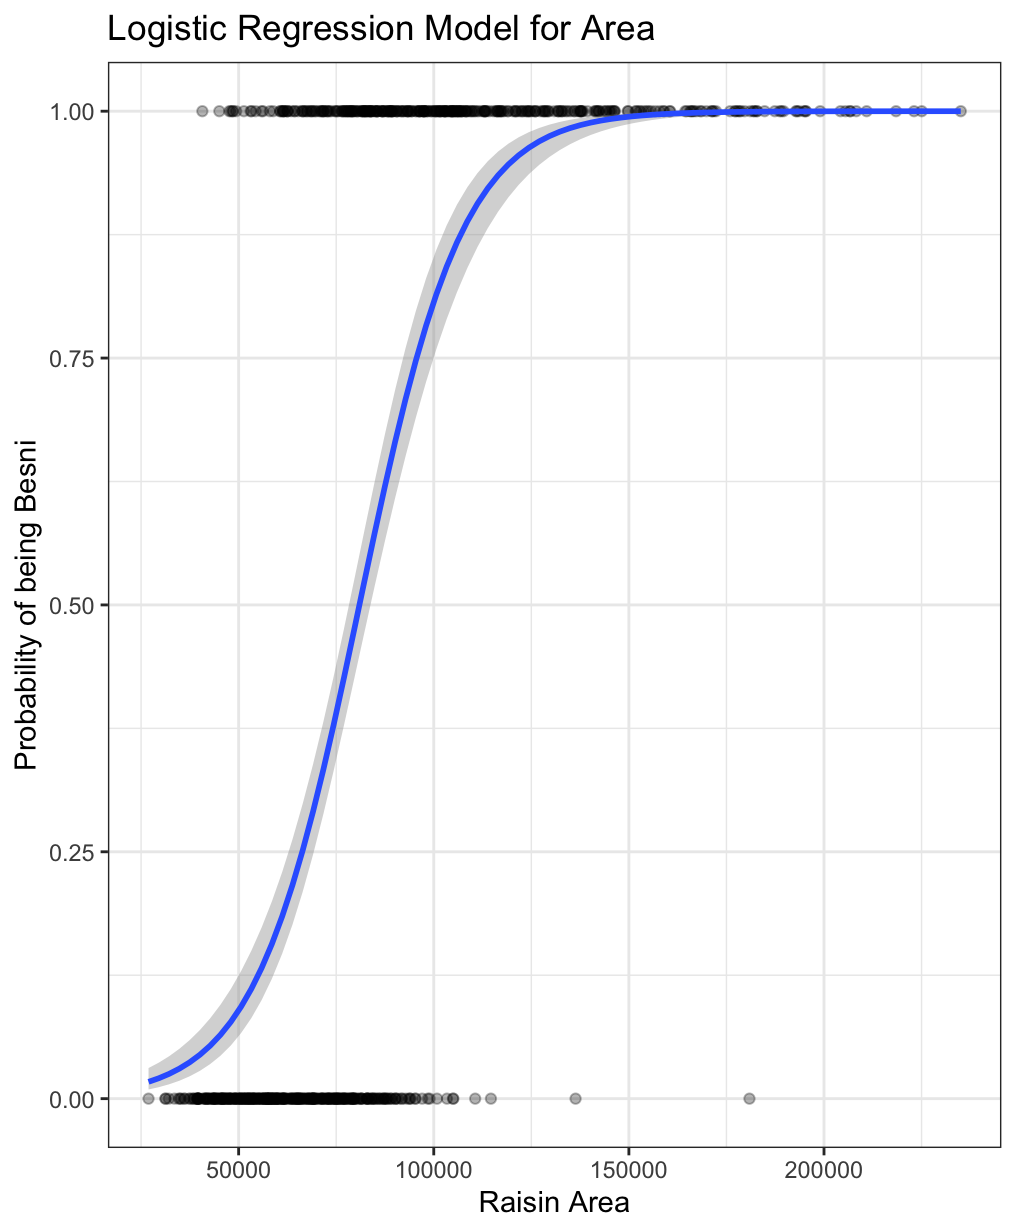
\includegraphics[width=\textwidth]{area_plot}
		\caption{Logistic regression model of the probability of being Besni as a function of raisin area.}
		\label{fig:area}
	\end{subfigure}
	\hfill
	\begin{subfigure}{0.4\textwidth}
		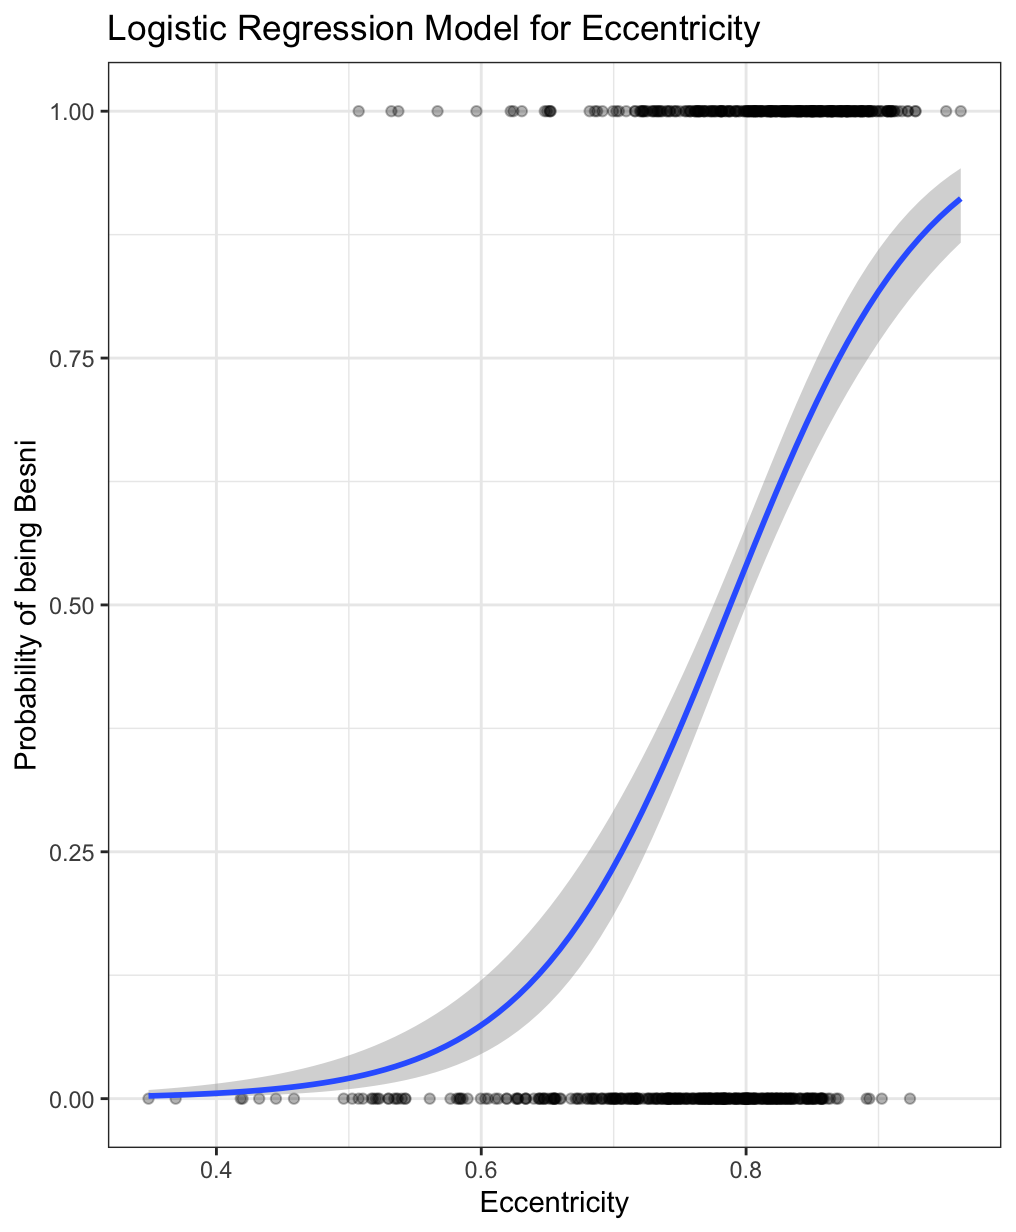
\includegraphics[width=\textwidth]{ecc_plot}
		\caption{Logistic regression model of probability of being Besni as function of eccentricity.}
		\label{fig:ecc}
	\end{subfigure}
	\caption{The slope of the area plot (figure \subref{fig:area}) being steeper than that of the eccentricity plot (figure \subref{fig:ecc}) indicates that area has a larger impact on the probability of the raisin being Besni, which is consistant with the coefficient table.}
	\label{fig:lr}
\end{figure}
Our diagonal plot for our model is shown in (Figure \ref{fig:diag})
\begin{figure}[!ht]
	\centering
	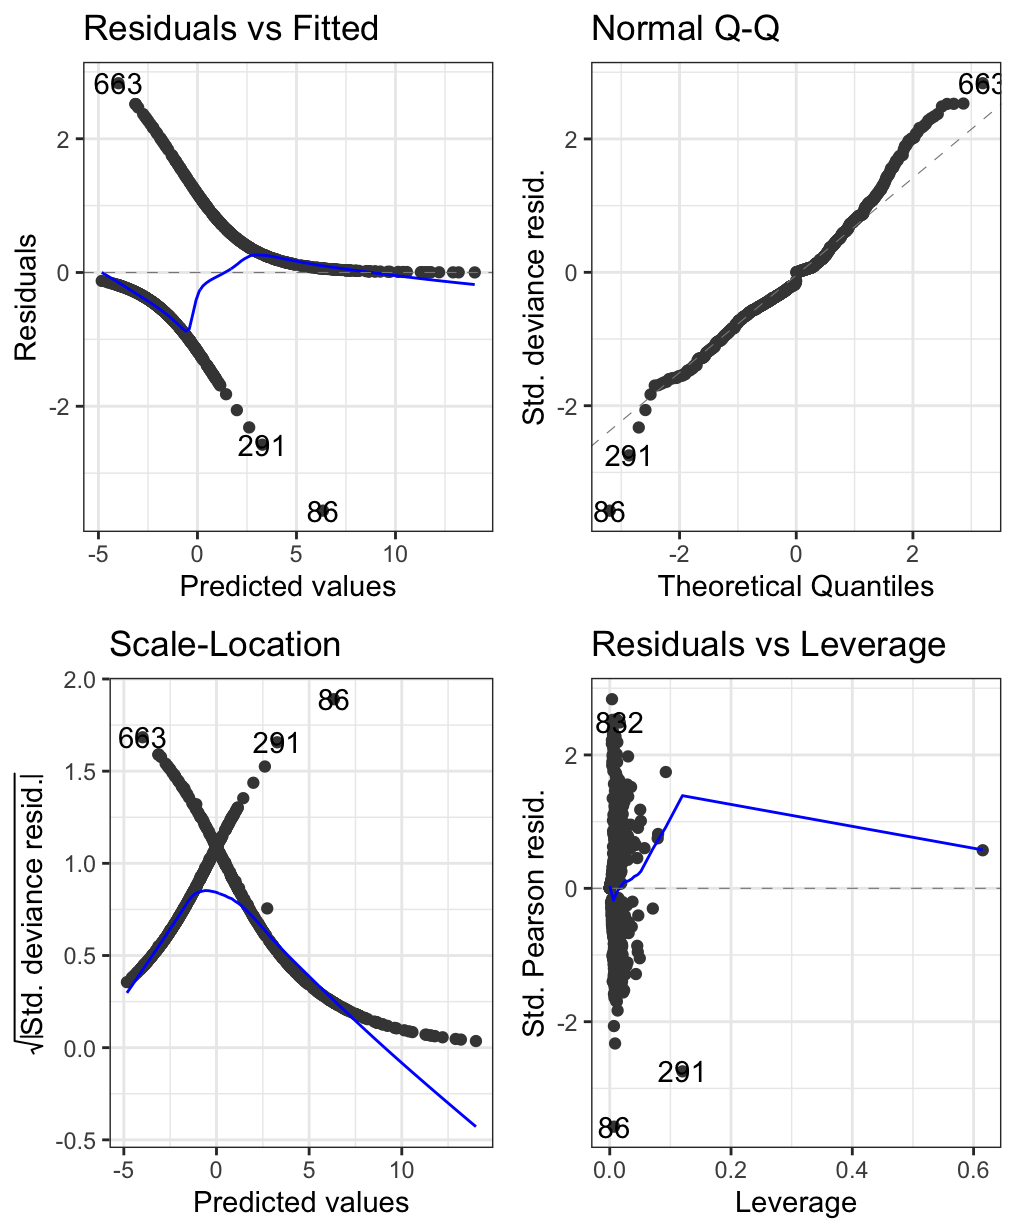
\includegraphics[width=0.5\textwidth]{diagonal_plots}
\caption{Diagonal plot for our model.}
\label{fig:diag}
\end{figure}

\clearpage
Clockwise from the top left(Figure \ref{fig:diag}):The Residual vs Fitted plot shows a clear pattern to the residuals and fitted points with an asymptote, so the model does not fit the data well.\\
The Normal Q-Q plot tells us that the data is normally distributed because the data mostly follows the $y=x$ line.\\
In the Scale-Location plot, the blue line is not horizontal and has a spike near 0 so the equal variance assumption is violated.\\
The Residual vs Leverage plot shows no high leverage points with large residuals. \\
The ROC curve is shown in Figure \ref{fig:roc}. With an AUC of 0.9434, the model does well at classifying observations as being more like Kecimen or Besni.
\begin{figure}[ht]
	\centering
	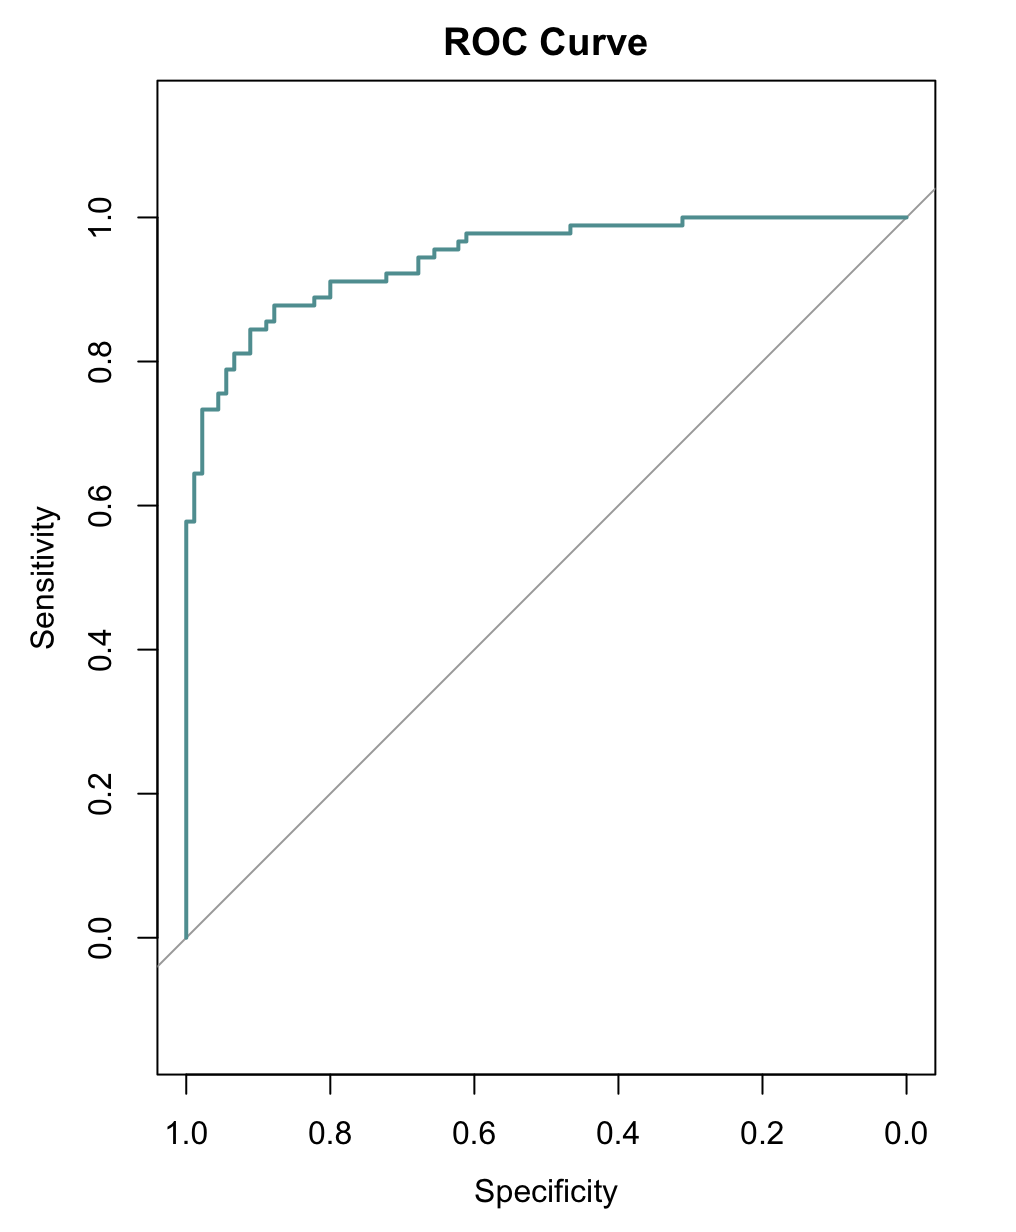
\includegraphics[width=0.75\textwidth]{roc_curve}
\caption{ROC curve for our model}
\label{fig:roc}
\end{figure} \\
Our code is on the next page:
\clearpage
\begin{verbatim}
# Load required libraries
library(caTools)
library(tidyverse)
library(caret)
library(ggplot2)
library(dplyr)
library(pROC)
library(ggfortify)

# Load data set
raisins <- read.csv("Raisin_Dataset.csv")
raisins <- na.omit(raisins) # Remove missing values

# Convert Class to binary (Besni = 1, Kecimen = 0)
raisins$Class <- ifelse(raisins$Class == "Besni", 1, 0)

# Shuffle data
set.seed(37)
raisins <- raisins[sample(nrow(raisins)), ]

# Split into training and test set
split <- sample.split(raisins$Class, SplitRatio = 0.8)

train <- subset(raisins, split == TRUE)
test <- subset(raisins, split == FALSE)

# Model
model <- glm(Class ~ Area + MajorAxisLength + MinorAxisLength + 
                 Eccentricity + ConvexArea + Extent + Perimeter, 
               data = train, 
               family = "binomial")

summary(model)

dev.new()
autoplot(model)

# Predictions
pred <- predict(model, test, type = "response")
pred_class <- ifelse(pred > 0.5, "Besni", "Kecimen")

# Confusion Matrix
conf_matrix <- table(Predicted = pred_class, Actual = test$Class)
print(conf_matrix)

train.data <- train %>%
  mutate(prob = predict(model, type = "response"))

dev.new()
area_plot <- ggplot(train.data, aes(x = Area, y = Class)) +
  geom_point(alpha = 0.3) +  
  geom_smooth(method = "glm", method.args = list(family = "binomial")) +
  labs(
    title = "Logistic Regression Model for Area",
    x = "Raisin Area",
    y = "Probability of being Besni"
  )

print(area_plot)

dev.new()
ecc_plot <- ggplot(train.data, aes(x = Eccentricity, y = Class)) +
  geom_point(alpha = 0.3) +  
  geom_smooth(method = "glm", method.args = list(family = "binomial")) +
  labs(
    title = "Logistic Regression Model for Eccentricity",
    x = "Eccentricity",
    y = "Probability of being Besni"
  )

print(ecc_plot)

# ROC curve
roc_curve <- roc(test$Class, pred)
dev.new()
plot(roc_curve, col = "cadetblue", main = "ROC Curve")
auc_value <- auc(roc_curve)
cat("AUC:", auc_value, "\n")

# Feature Importance
importance <- summary(model)$coefficients[, "Estimate"]
importance_df <- data.frame(Feature = names(importance), Estimate = importance)
dev.new()
ggplot(importance_df, aes(x = reorder(Feature, Estimate), y = Estimate)) +
  geom_bar(stat = "identity", fill = "pink") +
  coord_flip() +
  labs(title = "Feature Importance",
       x = "Feature",
       y = "Coefficient Estimate")
\end{verbatim}


\section{References}
We used the \texttt{Advertising.csv} dataset from Trevor Hastie’s “An Introduction to Statistical Learning”  GitHub page\footnote{https://trevorhastie.github.io/ISLR/Advertising.csv}.


\end{document}

